\documentclass{beamer}

\setbeameroption{hide notes} % Only slides
% \setbeameroption{show only notes} % Only notes
% \setbeameroption{show notes on second screen=right} % Both

% \usepackage{../AssertionEvidence.sty}
\usetheme{Madrid}
\usepackage{hyperref}
\usepackage{graphicx}
\usepackage{tikz}
\usepackage[style=verbose,backend=biber]{biblatex}

\defbeamertemplate*{title page}{customized}[1][]{
\begin{center}
  \usebeamerfont{title}\inserttitle\par
  \usebeamerfont{subtitle}\usebeamercolor[fg]{subtitle}\insertsubtitle\par
  \bigskip
  \usebeamerfont{author}\insertauthor\par
  \usebeamerfont{institute}\insertinstitute\par
  \usebeamerfont{date}\insertdate\par
  \usebeamercolor[fg]{titlegraphic}\inserttitlegraphic  
\end{center}  
}

\graphicspath{ {../imgs/} }

% Add above to the style

\title{Introduction to Artificial Intelligence}
\subtitle{The foundation and history of Artificial Intelligence and its Applications}
\author[RMS]{Rojesh Man Shikhrakar}

\begin{document}
\maketitle

\begin{frame}
  \frametitle{Syllabus: CACS410 Artificial Intelligence (3 Cr)}
  \begin{itemize}
    \item Introduction and Foundation of AI
    \item Problem Solving Methods: State space, Uninformed and Informed Search, Adversarial Search
    \item Knowledge Representation and Reasoning: Logic, and Uncertainty Quantification
    \item Machine Learning: Supervised, Unsupervised, Reinforcement Learning
    \item Neural Network and Natural Language Processing
    \item Expert System and Machine Vision
  \end{itemize}
\end{frame}

\begin{frame}
  \frametitle{Reference Books}
  \begin{columns}
    \begin{column}<1->{0.45\textwidth}
      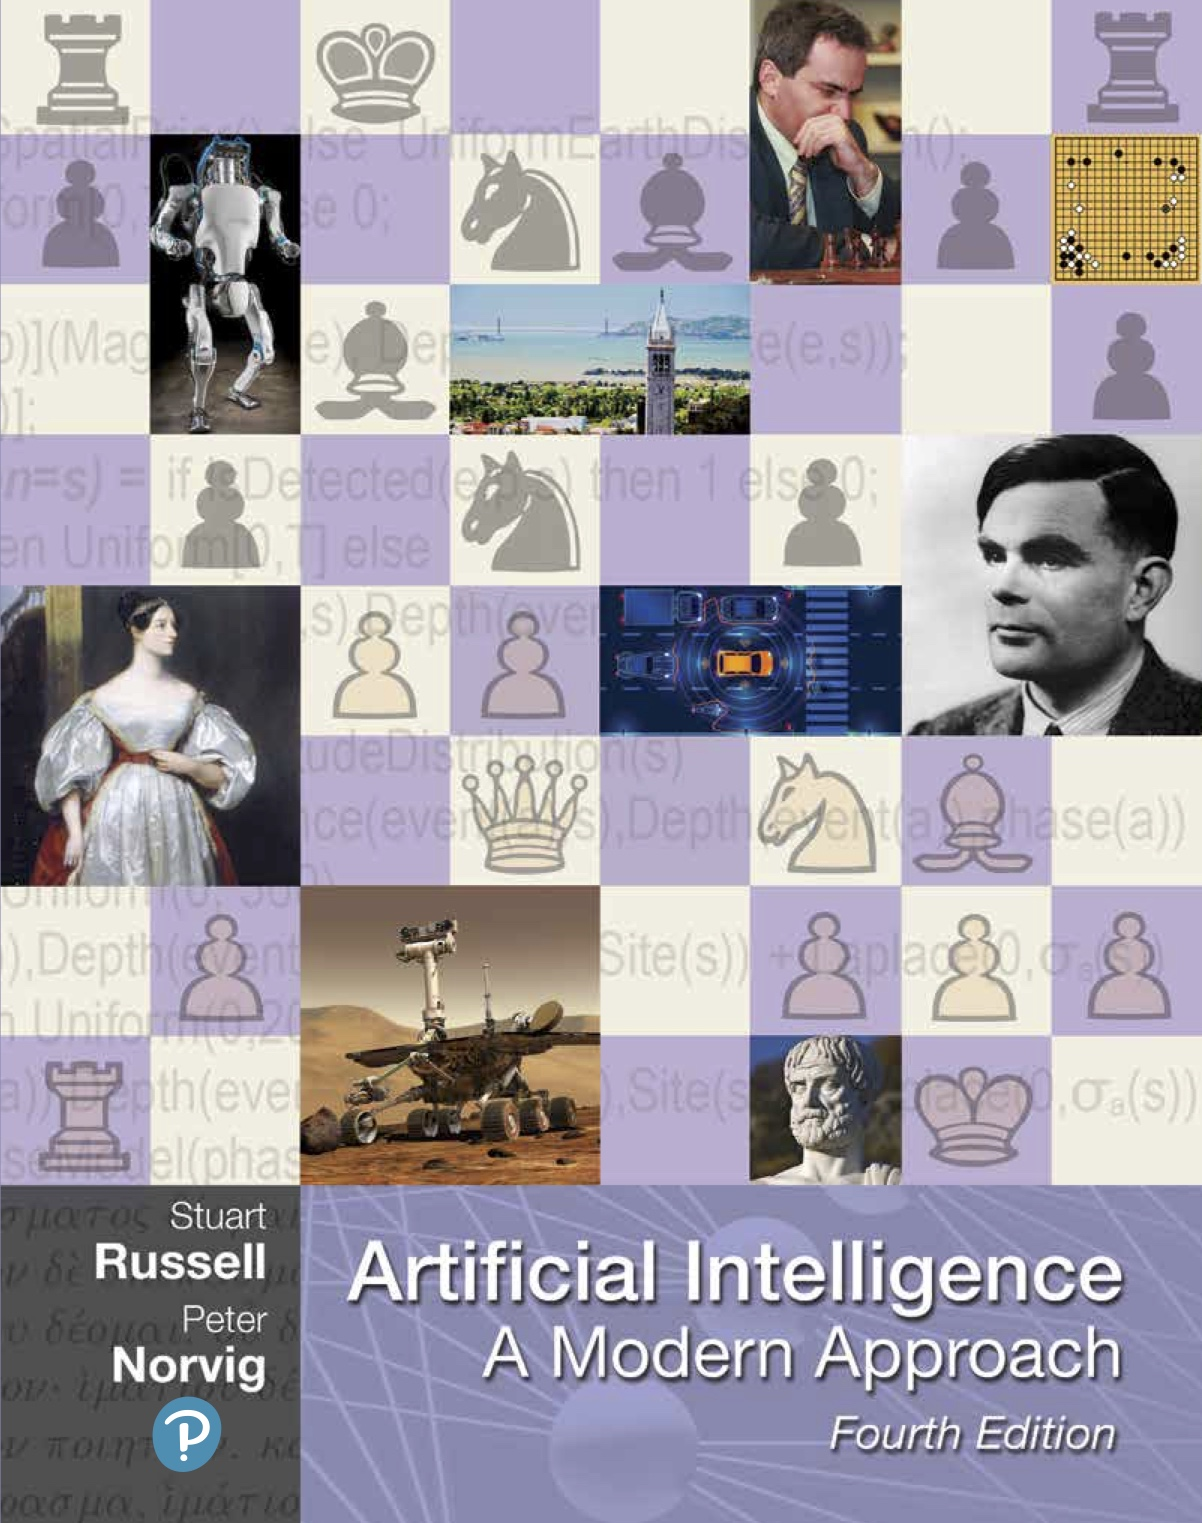
\includegraphics[width=0.8\textwidth]{AIMABook.png}
    \end{column}
    \begin{column}<2>{0.45\textwidth}
      Other Books
      \begin{itemize}
        \item E. Rich, K. Knight, Shivashankar B. Nair, Artificial Intelligence, Tata McGraw Hill.
        \item George F. Luger, Artificial Intelligence: Structures and Strategies for Complex Problem Solving, Benjamin/Cummings Publication
        \item D. W. Patterson, Artificial Intelligence and Expert Systems, Prentice Hall.
        \item P. H. Winston, Artificial Intelligence, Addison Wesley.
      \end{itemize}
    \end{column}
  \end{columns}
\end{frame}

\begin{frame}
  \frametitle{Syllabus: Unit 1: Introduction [6 Hrs]}
  \begin{itemize}
    \item 1.1 Intelligence, Intelligent behavior, Artificial Intelligence, Understanding Al based on thought process and behavior, Hard vs. Strong Al, Soft vs. Weak AI
    \item 1.2 Foundations of Al
    \item 1.3 Applications of Al
    \item 1.4 Intelligent Agents: Introduction of agents, Structure of Intelligent agent, Properties of Intelligent Agents, PEAS description of Agents, Types of Agents: Simple Reflexive, Model Based, Goal Based, Utility Based, Learning agent, Environment Types: Deterministic, Stochastic, Static, Dynamic, Observable, Semi-observable, Single Agent, Multi Agent
  \end{itemize}
\end{frame}

\begin{frame}
  \begin{quote}
    "We call ourselves *Homo sapiens* --man the wise-- because our intelligence is so important for us. For thousands of years, we have tried to understand how we think; that is, how a mere handful of matter can perceive, understand, predict and manipulate a world far larger and more complicated than itself. The field of artificial intelligence or AI, goes further still: it attempts not just to understand but also to build intelligent entities." 
  \end{quote}
  \raggedleft
    Artificial Intelligence, A Modern Approach \\
    by Stuart Russell and Peter Norvig    

\end{frame}

\begin{frame}
  \frametitle{Our perception of AI is mostly through movies, books and news}
  \begin{columns}
    \column[t]{0.35\textwidth}
    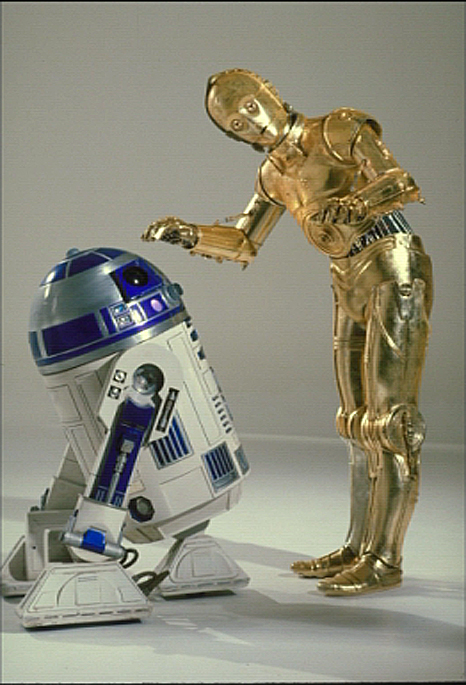
\includegraphics[width=\textwidth]{R2D2.png}
    \column[t]{0.65\textwidth}
    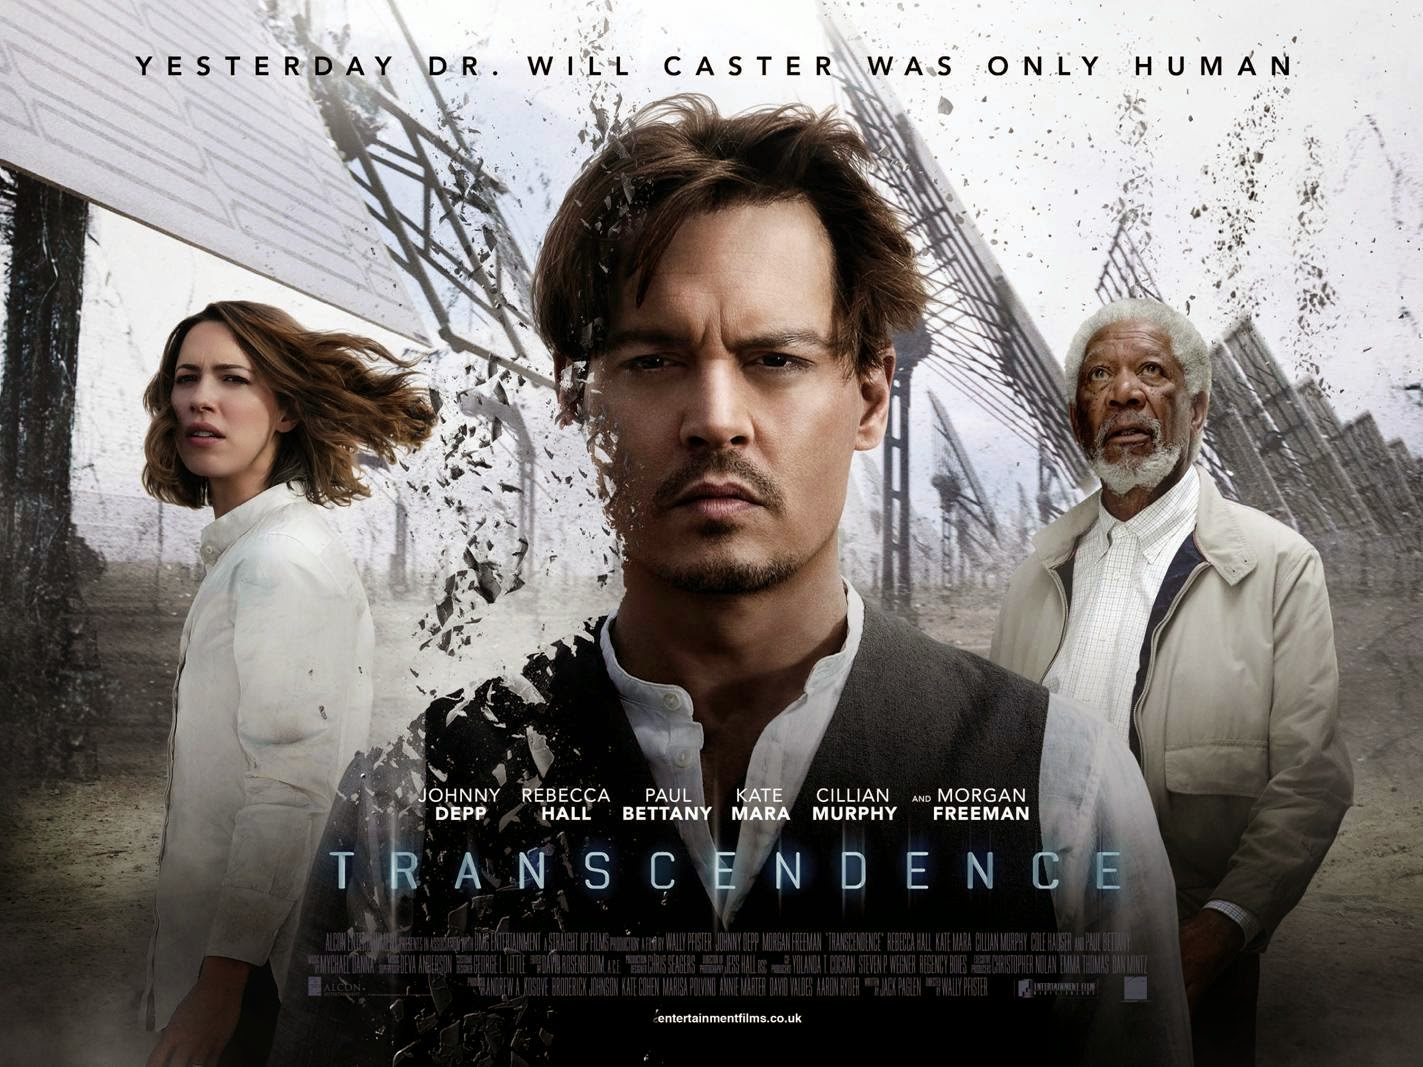
\includegraphics[width=\textwidth]{Transcedence.png}
  \end{columns}
\end{frame}

\begin{frame}
  \frametitle{AI in the Real world is much different}
  \begin{columns}
    \column{0.45\textwidth}
    \includegraphics[width=\textwidth]{FaceDetection.png}
    \column{0.45\textwidth}
    \begin{itemize}
      \item ChatGPT and Content Generation Tools
      \item Translate Langauges
      \item Speak Recognition
      \item Navigate through Digital Maps
      \item Drones to track you and record your videos
      \item Robotics Technologies: Sophia, Roomba, industrial robots
      \item And Many More ...
    \end{itemize}
  \end{columns}  

\end{frame}

\begin{frame}
  \frametitle{What does it mean to be Intelligent ?}
  \framesubtitle{The capacity for abstraction, logic, understanding, self-awareness, learning, emotional knowledge, reasoning, planning, creativity, critical thinking, and problem-solving}

  \begin{columns}
    \begin{column}<1->[t]{0.5\textwidth}
      How do scientists measure intelligence in animals ?
    \begin{itemize}
      \item Mirror-self Recognition: indicator of self-awareness
      \item Problem-solving ability: adaptive behavior or manipulate environment
      \item Number of neurons in the brain is a reliable indicator of animal Intelligence
      \item Self-Control: forgo eating for later
    \end{itemize}
    \end{column}

    \begin{column}<2>[t]{0.5\textwidth}
      7 Types of intelligence in human (Howard Gardner's Theory)
      \begin{itemize}
        \item Spatial : think abstractly in dimension
        \item Bodily-Kinesthetic: Physical and Athletic
        \item Musical: rythm, pitch, tone, melody, ...
        \item Logical-Mathematical: solve problems
        \item Linguistic: Language and communication
        \item Interpersonal: understanding others
        \item Intrapersonal: understanding onself
        
      \end{itemize}
      
    \end{column}
  \end{columns}
\end{frame}

\begin{frame}
  \frametitle{The Pursuit of Artificial Intelligence}
  \framesubtitle{Giving Machines ability to perform tasks normally associated with human Intelligence}

  \begin{itemize}
    \item AI in Myths and Stories from ancient civilization
    \item AI in Automation and Robotics
    \item Understanding human brain
    \item Developing Artificial Neural Network
    \item Computation Theory and making machine think
    \item Approaches to Artificial Intelligence so far
  \end{itemize}

\end{frame}

\begin{frame}
  \frametitle{In Greek mythology, the bronze giant Talos built by Hephaestus was tasked with protecting the island of Crete}  
  \begin{columns}
    \begin{column}<1->{0.5\textwidth}
      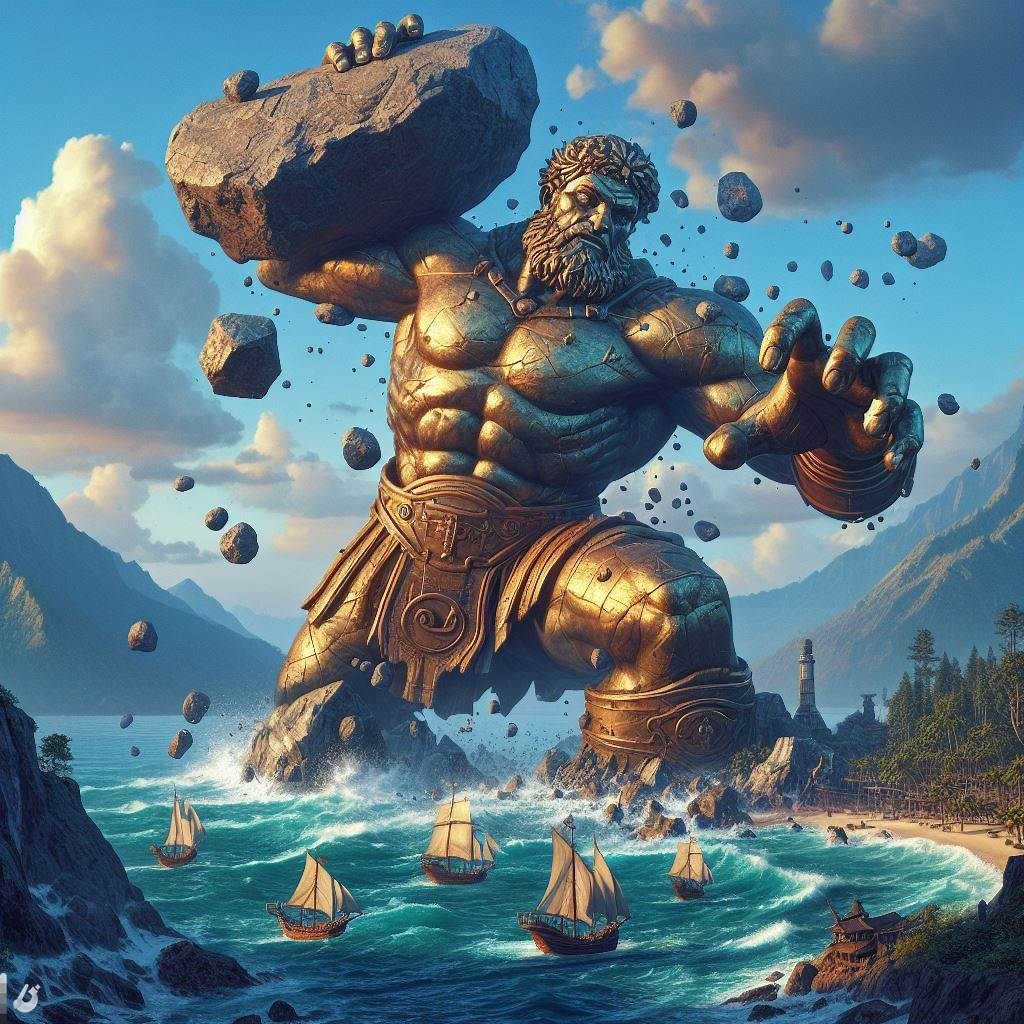
\includegraphics[width=\textwidth]{Talos_AIGen.jpeg}
    \end{column}
    \begin{column}<2>{0.5\textwidth}
      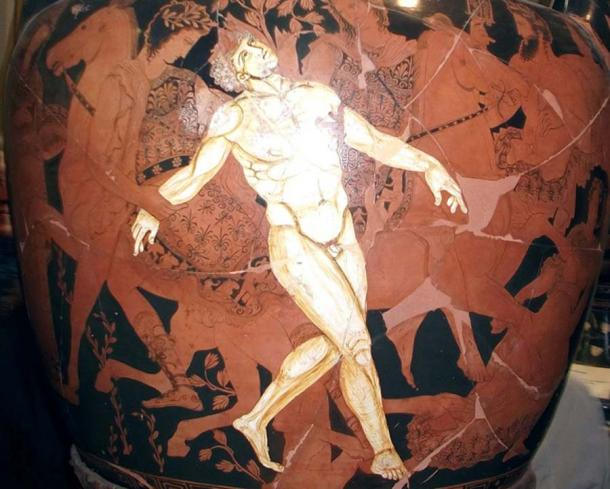
\includegraphics[width=\textwidth]{Talos_death.jpg}
      Source: \href{https://commons.wikimedia.org/wiki/File:Vaso_di_Talos_particolare.JPG}{Forzaruvo94}
    \end{column}
  \end{columns}
  
  \href{https://www.ancient-origins.net/myths-legends-europe/talos-00157}{Talos of Crete: A 2,000-Year-Old Tale of the First Robot God}

  \href{https://news.stanford.edu/2019/02/28/ancient-myths-reveal-early-fantasies-artificial-life/}{Myths and AI}

  \note{Talos was Bronze Giant built by In Greek Mythology (~700 BC), Talos was bronze giant build by Hephaestus, the Greek god of invention and blacksmithing,
   under commission by Zeus, the king of greek gods and was tasked with protecting the island of Crete.
  Talos stood guard over the island, tirelessly patrolling the shores three times a day and hurled massive boulders towards invading enemy ships.
  Talos had a tube running from his head to feet that carried a mysterious life-giving elixir called 'ichor'. 
  Later in another text sorceress Medea defeated Talos by removing a bolt of Talos ankle draining the ichor fluid. 
  Hephaestus also build an artificial evil woman sent to Earth with task to punish humans for discovering fire. 
  Hephaestus also created several young golden Maidens.}
\end{frame}

\begin{frame}
  \frametitle{AI \& Robotics in Hindu Mythology}
  \framesubtitle{Robots guarded Buddha's relics in a legend of ancient India "Lokapannatti"}

  \begin{columns}
    \begin{column}<1->{0.5\textwidth}
      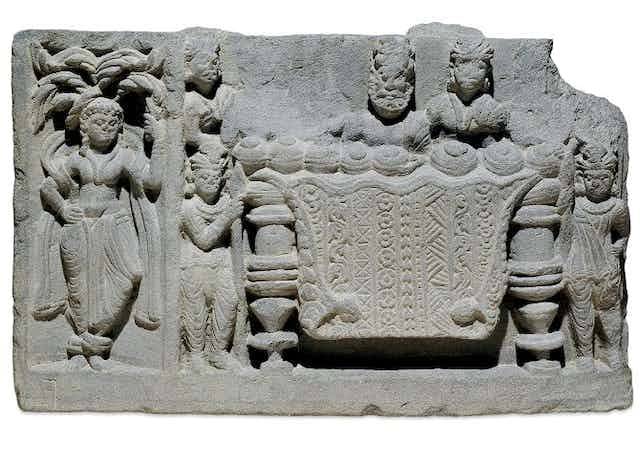
\includegraphics[width=\textwidth]{Buddha_Relic_Robots.jpg}
      Source:\href{https://theconversation.com/robots-guarded-buddhas-relics-in-a-legend-of-ancient-india-110078}{Robots guarded Buddha’s relics in a legend of ancient India}
    \end{column}
    \begin{column}<2>{0.5\textwidth}
      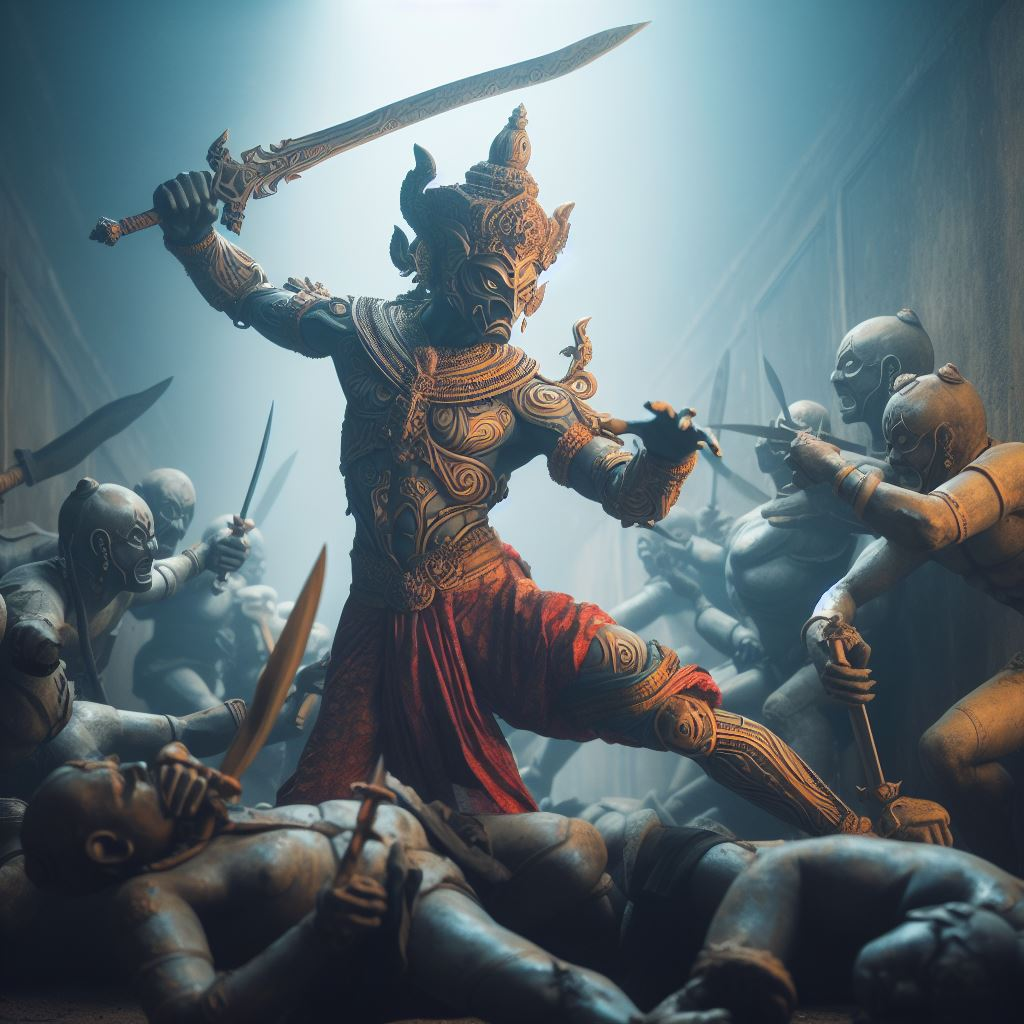
\includegraphics[width=\textwidth]{IndiaMythonRobot.jpeg}
    \end{column}
  \end{columns}
  
  \note{in Hindu mythology the Vishwakarma, the god of craftsmanship and the architect of gods, and the sorceress Maya had created automation along with many architectural wonders. Vishwakarma (meaning: world creator) is also regarded as the creator of the Brahma, Vishnu and Shiva.
  
  Furthemore, Indian Lokapannatti (collection of cycles and lores from 11 century AD), tells the story of how an army of automated soldiers (bhuta vahana yanta) were crafted to protect the relics of Buddha in a secret stupa.
  in the time of kings Ajatasatru and Asoka. Ajatasatru, who reigned from 492 to 460 B.C., was recognized for commissioning new military inventions, such as powerful catapults and a mechanized war chariot with whirling blades. 
  When Buddha died, Ajatasatru was entrusted with defending his precious remains. The king hid them in an underground chamber near his capital, Pataliputta (now Patna) in northeastern India.
  Traditionally, statues of giant warriors stood on guard near treasures. But in the legend, Ajatasatru's guards were extraordinary: They were robots. In India,
  automatons or mechanical beings that could move on their own were called "bhuta vahana yanta," or "spirit movement machines" in Pali and Sanskrit. According
  to the story, it was foretold that Ajatasatru's robots would remain on duty until a future king would distribute Buddha's relics throughout the realm.

  Two centuries after Ajatasatru, Asoka ruled the powerful Mauryan Empire in
  Pataliputta, 273-232 B.C\@. Asoka constructed many stupas to enshrine Buddha's
  relics across his vast kingdom. According to the legend, Asoka had heard the
  legend of the hidden relics and searched until he discovered the underground
  chamber guarded by the fierce android warriors. Violent battles raged between
  Asoka and the robots.
  }

\end{frame}

\begin{frame}
  \frametitle{Creating Automated Artificial Being (a Robot)}
  First recorded artificial automation was the steam-powered pigeon by Archytas of Tarentum (428 BC)

  \begin{columns}
    \begin{column}<1->{0.4\textwidth}
      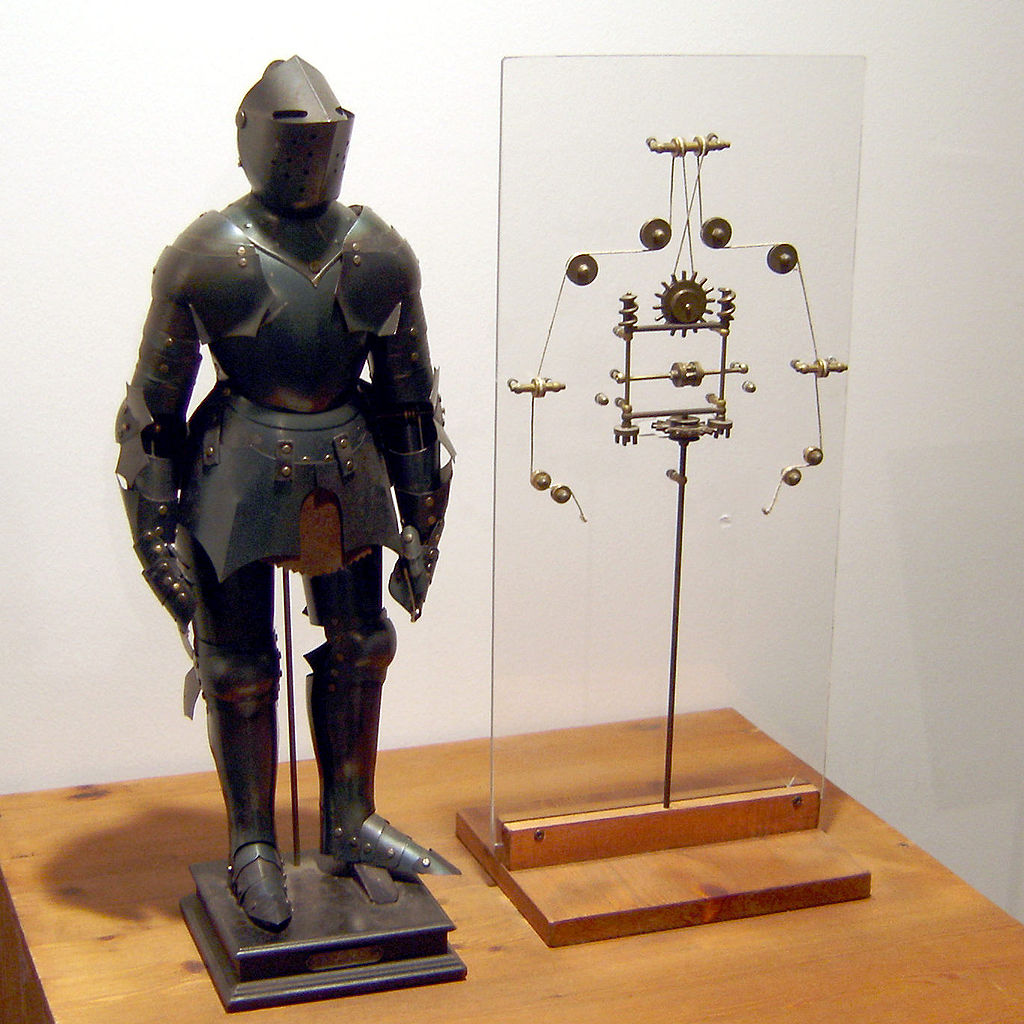
\includegraphics[width=\textwidth]{Leonardo-Robot.jpg}
      First verifiable automation is a humanoid knight ddrawn by Leonardo da Vinci in around 1495  
    \end{column}
    \begin{column}<2>{0.6\textwidth}
      \href{https://www.youtube.com/watch?v=-Xl2c91pWGc}{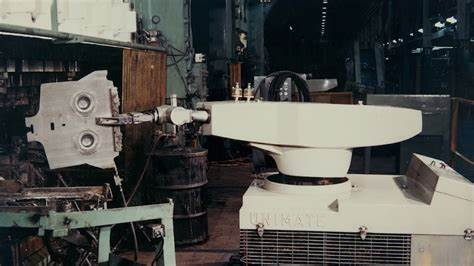
\includegraphics[width=\textwidth]{Unimate001.jpeg}}  
      "Unimate" was the first industrial robot developed by Joseph Engelberger (the Father of Robotics) in 1959
    \end{column}

  \end{columns}

\end{frame}

\begin{frame}
  \frametitle{Understanding Human Brain}
  \framesubtitle{Ancient civilization lacked adequate means to obtain knowledge about the human brain}
  \centering
  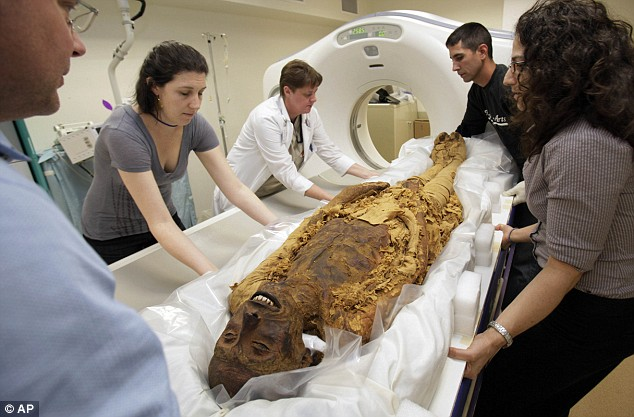
\includegraphics[width=0.7\textwidth]{EgyptianMummy.jpg}

  Source:\href{https://www.dailymail.co.uk/sciencetech/article-1195045/Ancient-Egyptians-unwrapped-CT-scans-reveal-secrets-beneath-bandages-2-000-year-old-mummies.html}{DailyMail}

  Ancient Egyptian regarded brain to be a form of "cranial stuffings" and had a vague recognition of the effect of head trauma.

  The heart was assumed to be the source of intelligence.
\end{frame}

\begin{frame}
  \frametitle{Understanding Human brain and the Discovery of Neurons}
  Alcmaeon (500 BC): brain was the organ that controlled the body.

  Galan (170 BC): theorized ventricles as site of thoughts.

  \begin{columns}
    \begin{column}<1>{0.4\textwidth}
    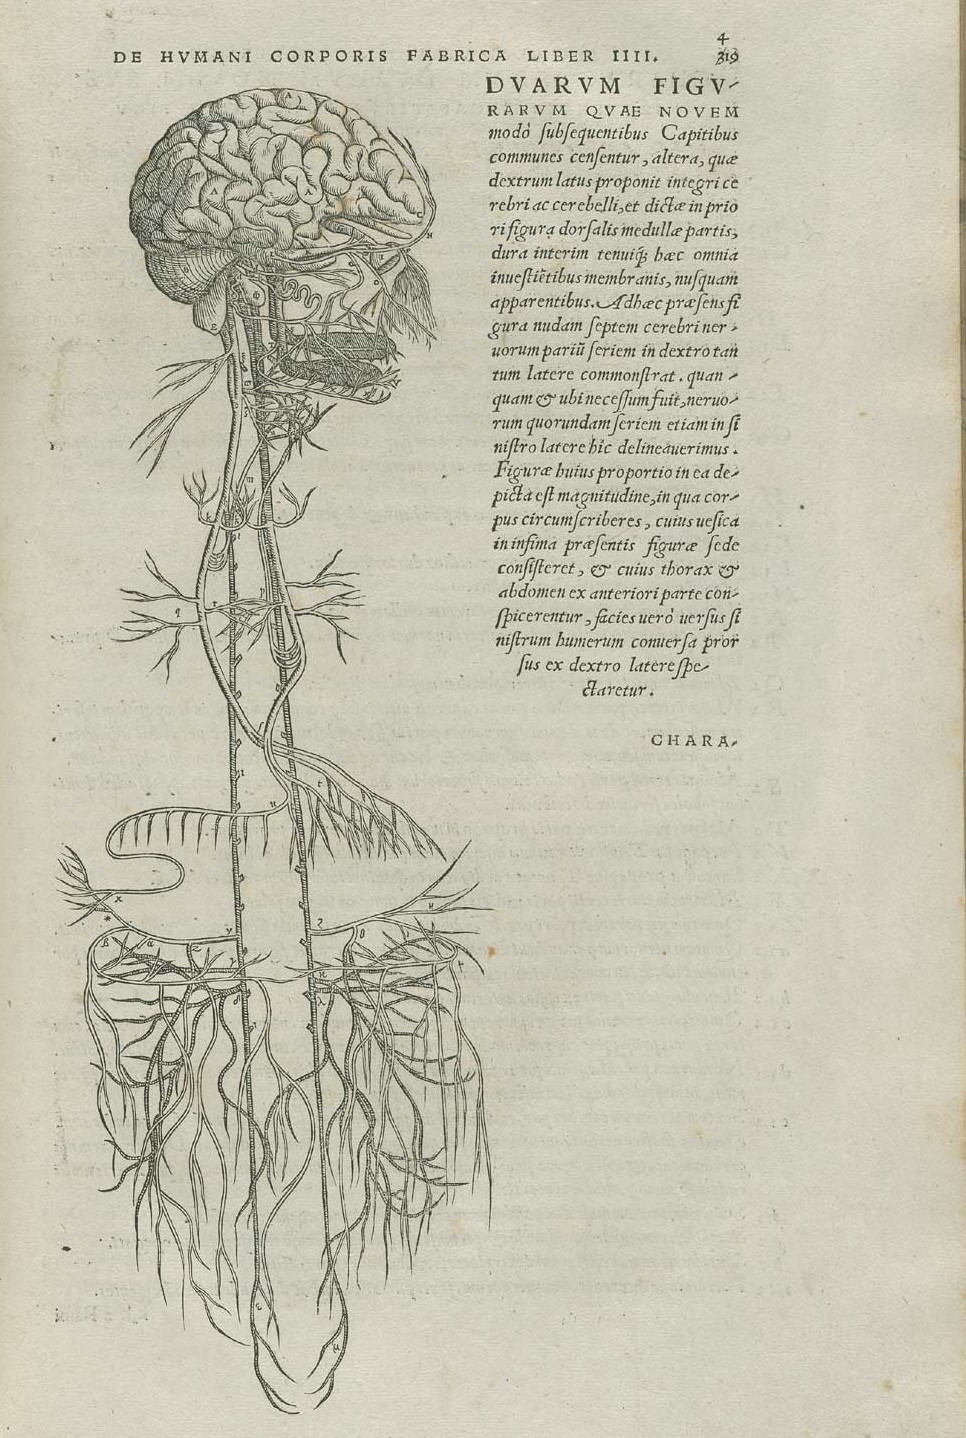
\includegraphics[width=0.8\textwidth]{Vesalius_Nerves.jpg}

    \small \href{https://www.nlm.nih.gov/exhibition/historicalanatomies/vesalius_home.html}{Andreas Vesalius: De corporis humani fabrica libri septem(1543)}
    \end{column}
    \begin{column}<2>{0.6\textwidth}
      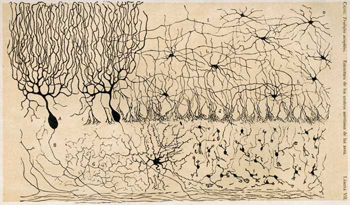
\includegraphics[width=\textwidth]{CajalCerebellum.jpg}
      Santiago RamÓn y Cajal and Camillo Golgi were awarded the 1906 Nobel Prize for their work on structure of nervous system that led to the neuron doctrine 
    \end{column}
  \end{columns}
  
  \note{
    \begin{itemize}
      \item Italian Luigi Galvani (1791) showed that electricity applied to nerves could make muscles contract
      \item Santiago Ramón y Cajal started investigating the nervous system in 1887 using the Golgi stain, that led to the formation of neuron doctrine (nervous sytem and brain are made up of discrete cells, neurons) for which Santiago RamÓn y Cajal and Camillo Golgi were awarded the 1906 Nobel Prize.
      \item In 1932 Sir Charles Sherrington and Edgar Adrian won the Nobel Prize for proposing the concept of synapses (junctions between neurons, pictured), which advanced the understanding of the central nervous system;
      \item Alan Hodgkin, Andrew Huxley and Australian Sir John Eccles won a Nobel Prize in 1963 for showing how neurons communicate via electrical and chemical signalling.
    \end{itemize}
  }

\end{frame}

\begin{frame}
  \frametitle{Modelling a Biological Neuron: Logical Calculus of Nervous Activity}
  \framesubtitle{Warren McCulloch and Walter Pitts (1943) attempted to model biological neurons as a binary threshold device that takes multiple binary inputs and produce a binary output}

  % #TODO

\end{frame}

\begin{frame}
  \frametitle{"Computing Machinery and Intelligence" by Alan Turing}
  
  \begin{columns}
    \column<1->{0.5\textwidth}
    
    \includegraphics[width=\textwidth]{"Alan-Turing.jpg"}
    
    \column<2>{0.5\textwidth}
    %#TODO
    \begin{itemize}
      \item The question whether machines can think itself is "meaningless"
      \item Prescribed a test "The Imitation Game" aka The Turing Test
      \item Critiques on Machines thinking ability
      \item Concept of Turing Machines (Digital Computer) 
    \end{itemize}
  \end{columns}
\end{frame}

\begin{frame}
  \frametitle{The Immitation Game aka The Turing Test}
  \framesubtitle{The interrogator, player C is asked to determine which player-A or B-is a human and which a computer}

  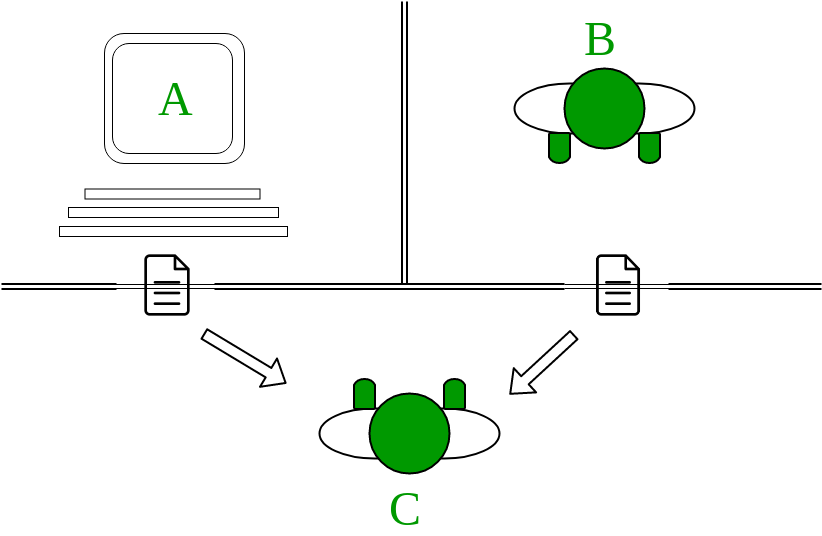
\includegraphics[width=\textwidth]{Turing-Test.png}

  \note{
   Natural language is rich in vocabulary and contextual meaning, There can be ambiguity, verbosity and impreciseness in the sentences. 
  }

\end{frame}

\begin{frame}
  \frametitle{Given the advances in NLP and advance conversational chatbots, Hector J. Levesque proposed a new test Winograd Schemas in 2012 }
  Book: Common Sesnse , the turing test and the quest for real AI.

  Winograd schema questions simply require the resolution of anaphora: the machine must identify the antecedent of an ambiguous pronoun

  Ask a pointed multiple choice question that requires knowledge of the subject matter.
  
  For eg: Context where "give" can appear are statistically quite similar to those where "receive" can appear, and yet the answer must change depending on which one is used.
  This helps make the test google-proof: having access to a large corpus of English test would likely not help.
  The claim is that doing better than guessing requires subject to figure out what is going on.



\end{frame}

\begin{frame}
  \frametitle{Dartmouth Conference 1956}
  \begin{columns}
    \column{0.4\textwidth}
    \includegraphics[width=\textwidth]{"Dartmouth-Summer-Conference-1956-proposal.jpeg"}    
    Source: \href{http://www-formal.stanford.edu/jmc/history/dartmouth.pdf}{Proposal for Conference}

    \column{0.6\textwidth}
    \includegraphics[width=\textwidth]{"Dartmouth-Summer-Conference-1956.jpeg"}    
    Source: \href{https://spectrum.ieee.org/dartmouth-ai-workshop}{IEEE Spectrum}

  \end{columns}

\end{frame}

\begin{frame}
  \frametitle{Dartmouth Conference Participants 1956}
  \begin{columns}
    \column{0.55\textwidth}
    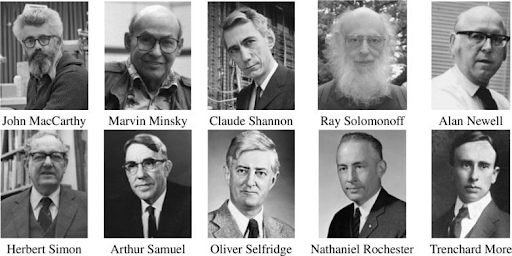
\includegraphics[width=\textwidth]{DarthmouthParticipants.png}    

    \column{0.45\textwidth}
    \begin{itemize}
      \item Shanon : Theory of Communication (1948)
      \item Arthur Samuel: Checker's program (1952)
      \item Newell \& Simon : Logic Theorist Proves theorems (1955) 
      \item Minsky with Dean Edmonds built first Neural Network Machine SNARC (1951)
      \item John McCarthy: coined the term AI (1955)
    \end{itemize}
  \end{columns}

\end{frame}

\begin{frame}
  \frametitle{Short History of AI}
  \small
  \begin{itemize}
    \item 1943: McCulloch \& Pitts: Boolean Circuit brain
    \item 1950: Turing's Computing Machiney and Intelligence paper
    \item 1950: Early AI Programs: chess, Checkers (RL), theorem proving
    \item 1956: Dartmouth meeting
    \item 1970s: Early development of Knowledge-based systems
    \item 1980s: Exper systems
    \item 1988-93: AI Winter
    \item 1990-2012: Staistical Approaches
    \item 2012: Deep Learning, Big Data and AI applications
    \item 2022: ChatGPT and hype of Large Language Models
  \end{itemize}
\end{frame}

\begin{frame}
  \frametitle{Approaches to Artificial Intelligence}
  \framesubtitle{Definition of AI based on the thought process/reasoning vs. behavior}
  Some defined Intelligence in terms of human performance other in formal definition as rationality (doing the "right" thing)
  \begin{tabular}{|c|c|}
    \hline
    \onslide<1->{\begin{minipage}{0.5\textwidth}
      \textbf{Thinking Humanly}

        Make computers think like humans
        
        Decision making, problem solving, learning
      \only<5>{Cognitive Science}
    \end{minipage}} &
    \onslide<2->{\begin{minipage}{0.5\textwidth}
      \textbf{Thinking Rationally}

      Study the mind functions (percive, reason, act) through computational models and Logics
      \only<5>{The Law of Thoughts}
    \end{minipage}} \\ 
    \hline
    \onslide<3->{\begin{minipage}{0.5\textwidth}
      \textbf{Acting Humanly}
      
      Perform actions that require intelligence
      \only<5>{Turing Test}
    \end{minipage}}&
    \onslide<4->{\begin{minipage}{0.5\textwidth}
      \textbf{Acting Rationally}

      Explain and emulate intelligent behaviors in terms of computational processes
      \only<5>{The Rational Agent}
    \end{minipage}} \\\hline
    \end{tabular}
  
\end{frame}

\begin{frame}
  \frametitle{Thinking Humanly: The Cognitive Science Approach}
  Based on 1960s cognitive revolution: information-processing psychology replaced prevailing behaviorism

Problem : requires scientific theories of internal activities of brain: what level of abstraction ?, how to validated ?

both approaches (cognitive science and cognitive neuroscience are now distinct from AI)

\end{frame}

\begin{frame}
  \frametitle{Thinking Rationally: Cognitive Modelling Approach}
   Normative (or prescritive) rather than descriptive

Based on several greek schools forms of logic: notation and rules of derivation for thoughts

Problem: not all intelligent behavior is mediated by logical deliberation, what is the purpose of thinking? what thought should I have?

\end{frame}

\begin{frame}
  \frametitle{Acting Humanly: Turing Test (Immitation Game) Approach}
  \begin{columns}
    \column{0.5\textwidth}
      Based on Turing (1950) "Computing Machinery and Intelligence"
      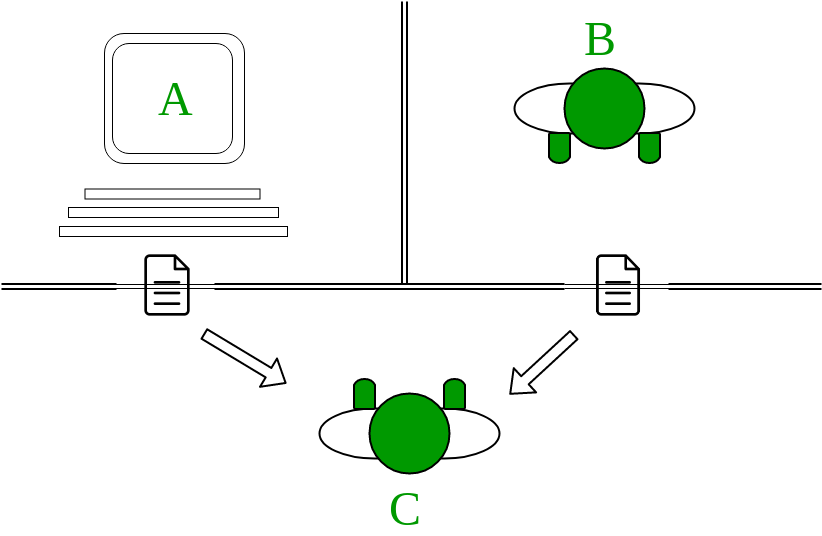
\includegraphics[width=\textwidth]{Turing-Test.png}
    \column{0.5\textwidth}
      Suggested Major Components of AI: Knowledge, Reasoning, Language Understanding, Learning
      \vspace{10pt}
      Problem: Turing test is not reproducible, constructive or amenable to mathematical analysis
  \end{columns}

\end{frame}

\begin{frame}
  \frametitle{Acting Rationally: The Rational Agent Approach}
  Rational behavior is about doing the right thing (that which expected to maximize goal achievement or utility given the available information)
  
  Problem: doesn't necessarily involve thinking reflex but instead think in the service of rational action

\end{frame}

\begin{frame}
  \frametitle{Foundation of AI}
  \framesubtitle{Disciplines that contributed ideas, views, techniques to AI}
  \begin{itemize}
    \item Philosophy: Logic, reasoning, foundation of learning, langauge,
    \item Mathematics: formal representation, Probability: Bayes Rule (1763), Stats: Maximum likelihood by Fisher (1992)
    \item Optimization: Stochastic Gradient Descent by Robbins/Monro (1951)
    \item Algorithms: UCS Dijkstra (1965)
    \item Psychology:  Adaptation, phenomena of percetion, motor control, experiment
    \item Economics: Minimax games by von Neumann (1944)
    \item Linguistics: First order logic by Frege (1893), Knowledge representation, grammar
    \item Neuroscience: Artificial Neural Networks (1943)
    \item Control Theory: value iteration by Bellman (1957), Stability,
    \item Least Square regression from astronomy by Gauss (1795)
  \end{itemize}
\end{frame}

\begin{frame}
  \frametitle{Category of AI: General (strong) AI \& Narrow (weak) AI}
  \framesubtitle{\textbf{Narrow AI} performs specific tasks within predefined contexts, while \textbf{General AI} can understand, learn, and apply its intelligence across a broad range of tasks like a human}

  \begin{columns}
    \column<1->{0.5\textwidth}
    \textbf{Narrow AI} perform a single task
    \begin{itemize}
      \item Face Recognition
      \item Self-driving car
      \item ChatGPT
    \end{itemize}

    \column<2>{0.5\textwidth}
    \textbf{General AI or Artificial General Intelligence (AGI)} Self-aware AI that can think, learn and act like humans
    \begin{itemize}
      \item Self-Aware Consciousness
      \item solve problems, learn and plan for future
      \item Challenges: 
    \end{itemize}
  \end{columns}
  
\end{frame}

% Section for Application
\begin{frame}
  \frametitle{What can AI do at present ? [Do a Web Search and find out]}
  \begin{itemize}
    \item Play a game of table tennis / Jeopardy / Dota
    \item Drive in Kathmandu's Traffic Jams, Nepal's Hilly Terrain
    \item Perform task based on human commands like "Go fetch the stapler"
    \item Perform a surgical operations
    \item Have a long conversation with a person
    \item Discover or prove a new Mathematical theorem ?
    \item Translate spoken langauges in realtime
    \item write an intentionally funny story
    \item Predict your future, who would be your spouse, \dots
    \item give competente legal advice in a specific area
  \end{itemize}

  Come up with a list of things AI cannot do currently, but could do in future
  \note{What is still missing 
  \begin{itemize}
    \item real understanding of Language
    \item integration learning with knowledgelong-range thinking at multiple levels of abstractions
    \item cumulative discovery of concepts and theories
  \end{itemize}
  }
\end{frame}

% \begin{frame}
%   \frametitle{The State of Language Understanding}
  
%   \begin{columns}
%     \column<1>{0.35\textwidth}
%     \begin{itemize}
%       \item Sentiment Analysis
%       \item Named Entity Recognition(NER)
%       \item Machine Translation
%       \item Information Extraction
%       \item Text Summarization
%       \item Question Answering
%       \item Chatbots \& Virtual Assitants
%       \item Semantic Search
%     \end{itemize}
  
%     \column<2>{0.3\textwidth}
%     OpenAI GPT-4 and other Language Models
%     Multilingual Language Models
    
%     \column<3>{0.3\textwidth}

  
%   \end{columns}

% \end{frame}

% \begin{frame}
%   \frametitle{State of Computer Vision and Image Generation}

%   \begin{columns}
%     \column<1>{0.3\textwidth}
%     \begin{itemize}
%       \item GANs
%       \item Diffusion Models
%       \item Foundation Models
%     \end{itemize}
%     \column<2>{0.3\textwidth}
    
%   \end{columns}

% \end{frame}

% \begin{frame}
%   \frametitle{State of Speech Recognition}

%   \begin{columns}
%     \column<1>{0.3\textwidth}
  
%     \column<2>{0.3\textwidth}
  
    
%     \column<3>{0.3\textwidth}
%     \href{https://www.youtube.com/watch?v=JvbHu_bVa_g}{Google's Personal Assistant making a reservation}  
  
%   \end{columns}

% \end{frame}

% \begin{frame}
%   \frametitle{State of Planning and Problem Solving}

%   \begin{columns}
%     \column<1>[t]{0.5\textwidth}
%     Maps and Navigation

%     \column<1>[t]{0.5\textwidth}
%     Games
    
%   \end{columns}

% \end{frame}

% \begin{frame}
%   \frametitle{State of Robotics}

%   \begin{columns}
%     \column<1>{0.3\textwidth}
%     \begin{itemize}
%       \item Worker robots
%       \item Soft Robots
%       \item Reconfigurable and Modular Robots
%       \item Surgical Robots
%       \item Foundational Models for Robotics
%     \end{itemize}
%     \href{https://ubuntu.com/blog/the-state-of-robotics-2022-review}{Robotics in 2022}
  
%     \column<2>{0.3\textwidth}

%   \end{columns}
  

% \end{frame}

\begin{frame}
  \frametitle{An Agent is an entiy that perceives, plan and acts}
  \framesubtitle{Agent perceives its environment through sensors and acts upon it through actuators}
  \begin{columns}
    \begin{column}{0.55\textwidth}

      \tikzset{every picture/.style={line width=0.75pt}} %set default line width to 0.75pt        
      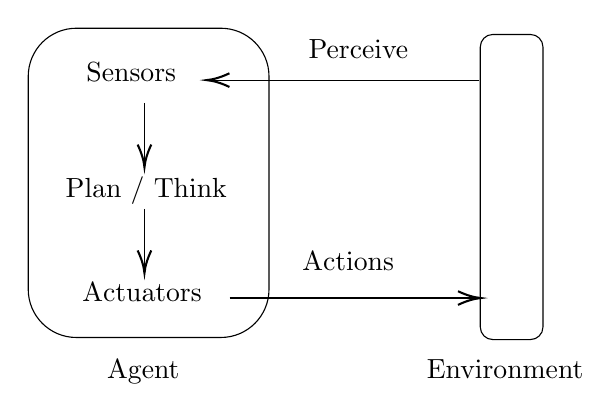
\begin{tikzpicture}[x=0.75pt,y=0.75pt,yscale=-1,xscale=1]
      %uncomment if require: \path (0,300); %set diagram left start at 0, and has height of 300

      %Rounded Rect [id:dp7065715939596047] 
      \draw   (13.2,78.8) .. controls (13.2,65.99) and (23.59,55.6) .. (36.4,55.6) -- (106,55.6) .. controls (118.81,55.6) and (129.2,65.99) .. (129.2,78.8) -- (129.2,181.4) .. controls (129.2,194.21) and (118.81,204.6) .. (106,204.6) -- (36.4,204.6) .. controls (23.59,204.6) and (13.2,194.21) .. (13.2,181.4) -- cycle ;
      %Rounded Rect [id:dp1683263044072274] 
      \draw   (231,64.64) .. controls (231,61.3) and (233.7,58.6) .. (237.04,58.6) -- (255.16,58.6) .. controls (258.5,58.6) and (261.2,61.3) .. (261.2,64.64) -- (261.2,199.56) .. controls (261.2,202.9) and (258.5,205.6) .. (255.16,205.6) -- (237.04,205.6) .. controls (233.7,205.6) and (231,202.9) .. (231,199.56) -- cycle ;
      %Straight Lines [id:da270942443985861] 
      \draw    (230.2,80.6) -- (101.2,80.6) ;
      \draw [shift={(99.2,80.6)}, rotate = 360] [color={rgb, 255:red, 0; green, 0; blue, 0 }  ][line width=0.75]    (10.93,-3.29) .. controls (6.95,-1.4) and (3.31,-0.3) .. (0,0) .. controls (3.31,0.3) and (6.95,1.4) .. (10.93,3.29)   ;
      %Straight Lines [id:da6260748217123768] 
      \draw    (110.2,185.6) -- (229.2,185.6) ;
      \draw [shift={(231.2,185.6)}, rotate = 180] [color={rgb, 255:red, 0; green, 0; blue, 0 }  ][line width=0.75]    (10.93,-3.29) .. controls (6.95,-1.4) and (3.31,-0.3) .. (0,0) .. controls (3.31,0.3) and (6.95,1.4) .. (10.93,3.29)   ;
      %Straight Lines [id:da6008479407887466] 
      \draw    (69.2,91.6) -- (69.2,120.6) ;
      \draw [shift={(69.2,122.6)}, rotate = 270] [color={rgb, 255:red, 0; green, 0; blue, 0 }  ][line width=0.75]    (10.93,-3.29) .. controls (6.95,-1.4) and (3.31,-0.3) .. (0,0) .. controls (3.31,0.3) and (6.95,1.4) .. (10.93,3.29)   ;
      %Straight Lines [id:da059574811068754396] 
      \draw    (69.2,142.6) -- (69.2,171.6) ;
      \draw [shift={(69.2,173.6)}, rotate = 270] [color={rgb, 255:red, 0; green, 0; blue, 0 }  ][line width=0.75]    (10.93,-3.29) .. controls (6.95,-1.4) and (3.31,-0.3) .. (0,0) .. controls (3.31,0.3) and (6.95,1.4) .. (10.93,3.29)   ;

      % Text Node
      \draw (204,214) node [anchor=north west][inner sep=0.75pt]   [align=left] {Environment};
      % Text Node
      \draw (50,214) node [anchor=north west][inner sep=0.75pt]   [align=left] {Agent};
      % Text Node
      \draw (40,71) node [anchor=north west][inner sep=0.75pt]   [align=left] {Sensors};
      % Text Node
      \draw (38,177) node [anchor=north west][inner sep=0.75pt]   [align=left] {Actuators};
      % Text Node
      \draw (147,60) node [anchor=north west][inner sep=0.75pt]   [align=left] {Perceive};
      % Text Node
      \draw (144,162) node [anchor=north west][inner sep=0.75pt]   [align=left] {Actions};
      % Text Node
      \draw (30,126) node [anchor=north west][inner sep=0.75pt]   [align=left] {Plan / Think};
      \end{tikzpicture}


      Agent Function maps from percept histories to actions $f: P \rightarrow A$
      
      Visualize: Games (Tetris, Chess), Robotic Vacuum Cleaner, \dots
    \end{column}
    \begin{column}{0.45\textwidth}
      \small
      \begin{itemize}
        \item Sensors: Keyboard, Camera, Accelerometer, \dots
        \item Vision, Audio, Tactile, Smell, Proprioception
        \item Actuators: motors, lights, monitors, speakers, \dots
        \item Planing step processes sensors data (signal processing, planning/reasoning system, motor control)
        \item A Rational Agent selects actions that maximizes its expected Utility
        \item An agent can learn to choose and apply techniques appropriate for each problem
      \end{itemize}
    \end{column}
  \end{columns}
  \note{Are Pocket Calculators Agents? Yes, Key state are sensors, Digit display is actuator, it does some processing from the sensors to give output
  
  However AI is more interested in agents with large computational resources and environments that require nontrivial decision making.
  
  Usually Program are persistent, autonomous, proactive and goal directed.
  }
  
\end{frame}

\begin{frame}
  \frametitle{Rational agent chooses actions to maximize the expected value of the performance measure}
  \framesubtitle{Performance measure evaluates the environment state or sequences}
  What should be the perform measure for the following

  \begin{itemize}
    \item Tetris Game : +100 for line clear, +800 for 4 line clear at once(Tetris), +1200 back-to-back (Tetris)
    \item Pacman : -1 per step, +10 food, +500 win, -500 die, +200 eat scared ghost
    \item Chess:
  \end{itemize}
  
  Rational Agents aren't omniscient (doesn't know everything), aren't clairvoyant (cannot perceive events in the future or beyond what's visible), but they can explore the environment and learn autonomously.

\end{frame}

\begin{frame}
  \frametitle{PEAS Framework: Eg Self Driving Car}
  \framesubtitle{Alternatively: PAGE (Percepts, Actions, Goals, Environment)}
  \begin{itemize}
    \item \textbf{P}erformance measure: distance traveled
    \item Sometimes \textbf{G}oal is used Objectives to achieve: destination reached, safety, \dots
    \item \textbf{E}nvironment: Nepal Street with other cars, Weather
    \item \textbf{A}ctuators: Steering, Break, Accelerator, Clutch, sidelights,\dots
    \item \textbf{S}ensors: Camera, Radar, Accelerometer, Engine Sensor, GPS, Microphone, \dots
  \end{itemize}

  Practice PEAS framework for 
  \begin{itemize}
    \item Tetris, Pac-Man, Chess
    \item Vacuum Robot
    \item Speech Translation
    \item Medical Diagnositc System
  \end{itemize}

\end{frame}

\begin{frame}
  \frametitle{Environment type can largerly determine the agent design}
  \begin{itemize}
    \item \textbf{Accessible}: Fully Observable vs Partially Observable: requires memory (internal state)
    \item Single-agent or Multiagent: compete or coordinate with other agents
    \item \textbf{Deterministic} or \textbf{Stochastic}: need to handle Uncertainty and contingencies
    \item Static or Dynamic: compute a rational decision (static)
    \item Discrete or Continuous : controller to be operated continuously or in discrete steps
    \item Known/unknown physics : need for exploration
    \item Known/unknown perf. measure: observe/interact with human supervisor
    \item Sequential or Episodic (current action will not effect future action): 
  \end{itemize}
  The real worlds is oftern inaccessible or partially observable, stochastic, sequential, dynamic and continuous.
\end{frame}

\begin{frame}
  \frametitle{Types of Agent based on its Thinking/Planning ability}
  "Low-level Intelligence" \hfill "High-level Intelligence"
  \rule{\textwidth}{2pt}
  \vspace{10pt}

  \begin{columns}
    \small
    \column{0.25\textwidth}
    \textbf{Simple Reflex Agents}

    Based on dofrect mapping from state to action, can be 
    \begin{itemize}
      \item conditional rules
      \item input-action tables
      \item Neural Network best action (no learning)
    \end{itemize}

    \column{0.25\textwidth}
    \textbf{Reflex Agents with internal state}

    Maintain an internal state
    \begin{itemize}
      \item Search problems
      \item Adversarial Games
      \item MDPs
    \end{itemize}

    \column{0.25\textwidth}
    \textbf{Goal-based Agents}

    Use Goals to index actions but cannot handle tradeoffs among goals
    \vspace{5pt}

    \textbf{Variables-based Agents}
  
    solve problems with soft or hard constraints or dependencies
    \begin{itemize}
      \item CSP
      \item Bayes Nets
    \end{itemize}

    \column{0.25\textwidth}
    \textbf{Utility-based agents}

    Compute expected value for an actions, handle tradeoffs and Uncertainty
    \vspace{5pt}

    \textbf{Logic-based agents}
    Use Natural Language, Reason deeply with Information
    
  \end{columns}
\end{frame}

\begin{frame}
  \frametitle{Representation spectrum based on the complexity of the problem}
  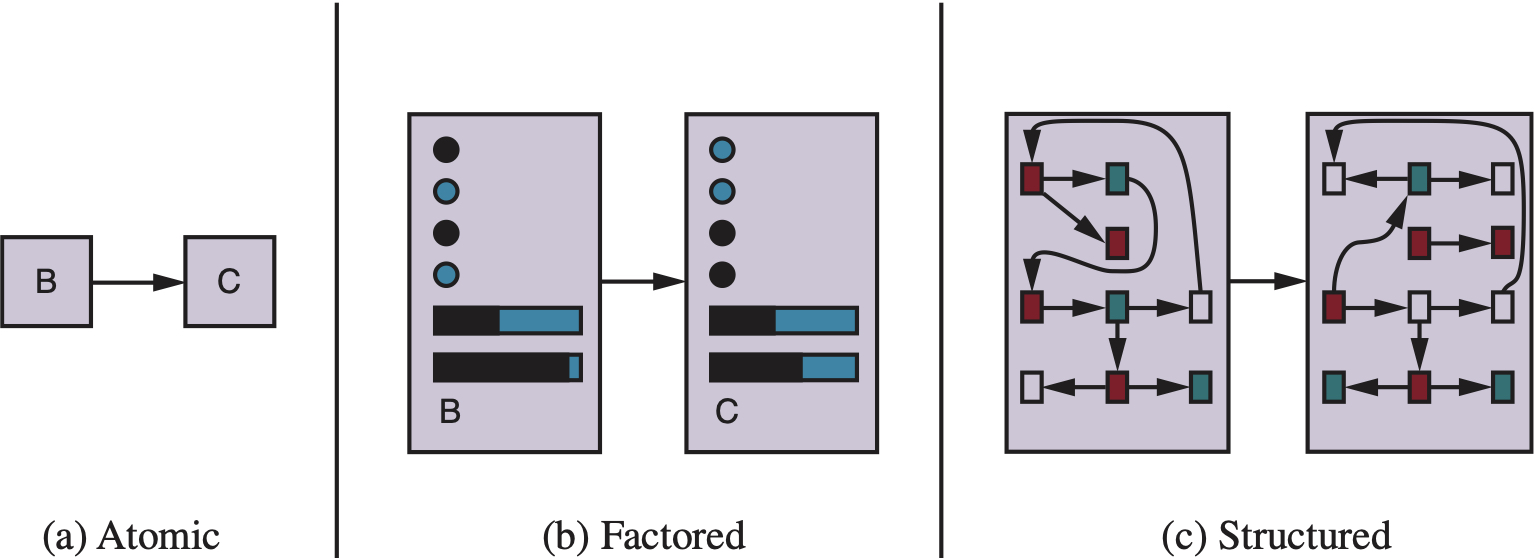
\includegraphics[width=\textwidth]{RepresentationSpectrum.png}
  \begin{columns}
    \small
    \column{0.27\textwidth}
    individual elements (B and C) have a direct connection or interaction

    \column{0.34\textwidth}
    elements (B and C) are not isolated but are part of a larger structure with additional component

    \column{0.34\textwidth}
    highly intricate network of interactions among multiple elements within a system.

  \end{columns}

  \note{
    \begin{itemize}
      \item Atomic (a): individual elements (B and C) have a direct connection or interaction. It's like a basic building block in a system.
      \item Factored (b):  shows elements (B and C) as part of a larger structure with additional components. It suggests that the elements are not isolated but interact with other parts of the system.
      \item Structured (c):  It depicts a highly intricate network of interactions among multiple elements within a system. It indicates that the elements are interconnected in various ways, forming a complex structure
    \end{itemize}}
\end{frame}

\begin{frame}
  \frametitle{Contents covered in this course}

\tikzset{every picture/.style={line width=0.75pt}} %set default line width to 0.75pt        

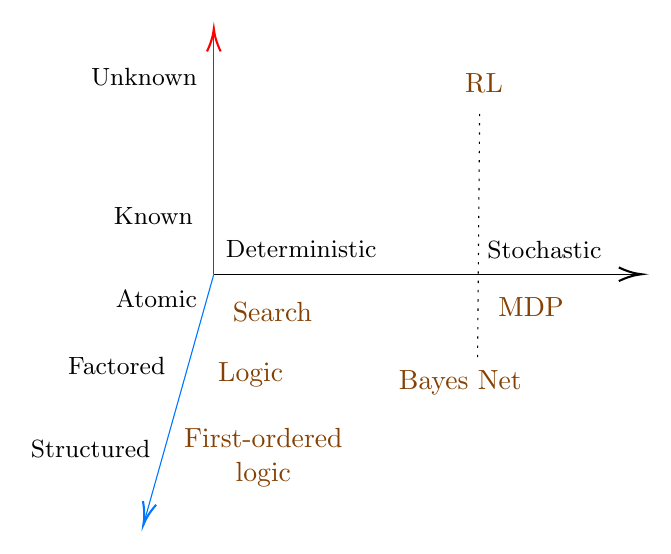
\begin{tikzpicture}[x=0.75pt,y=0.75pt,yscale=-1,xscale=1]
%uncomment if require: \path (0,300); %set diagram left start at 0, and has height of 300

%Straight Lines [id:da1337000113318687] 
\draw    (91.14,126.9) -- (295.2,126.9) ;
\draw [shift={(297.2,126.9)}, rotate = 180] [color={rgb, 255:red, 0; green, 0; blue, 0 }  ][line width=0.75]    (10.93,-3.29) .. controls (6.95,-1.4) and (3.31,-0.3) .. (0,0) .. controls (3.31,0.3) and (6.95,1.4) .. (10.93,3.29)   ;
%Straight Lines [id:da6549122301713701] 
\draw [color={rgb, 255:red, 0; green, 119; blue, 255 }  ,draw opacity=1 ]   (91.14,126.9) -- (57.74,245.67) ;
\draw [shift={(57.2,247.6)}, rotate = 285.71] [color={rgb, 255:red, 0; green, 119; blue, 255 }  ,draw opacity=1 ][line width=0.75]    (10.93,-3.29) .. controls (6.95,-1.4) and (3.31,-0.3) .. (0,0) .. controls (3.31,0.3) and (6.95,1.4) .. (10.93,3.29)   ;
%Straight Lines [id:da20729140677781333] 
\draw [color={rgb, 255:red, 255; green, 0; blue, 0 }  ,draw opacity=1 ]   (91.14,126.9) -- (91.14,10.6) ;
\draw [shift={(91.14,8.6)}, rotate = 90] [color={rgb, 255:red, 255; green, 0; blue, 0 }  ,draw opacity=1 ][line width=0.75]    (10.93,-3.29) .. controls (6.95,-1.4) and (3.31,-0.3) .. (0,0) .. controls (3.31,0.3) and (6.95,1.4) .. (10.93,3.29)   ;
%Straight Lines [id:da11852321652256204] 
\draw  [dash pattern={on 0.84pt off 2.51pt}]  (219.2,49.6) -- (218.2,168.6) ;

% Text Node
\draw (95.72,109.59) node [anchor=north west][inner sep=0.75pt]  [font=\small] [align=left] {Deterministic};
% Text Node
\draw (221.72,109.59) node [anchor=north west][inner sep=0.75pt]  [font=\small] [align=left] {Stochastic};
% Text Node
\draw (41.72,93.59) node [anchor=north west][inner sep=0.75pt]  [font=\small] [align=left] {Known};
% Text Node
\draw (30.72,26.59) node [anchor=north west][inner sep=0.75pt]  [font=\small] [align=left] {Unknown};
% Text Node
\draw (42.72,133.59) node [anchor=north west][inner sep=0.75pt]  [font=\small] [align=left] {Atomic};
% Text Node
\draw (19.72,165.59) node [anchor=north west][inner sep=0.75pt]  [font=\small] [align=left] {Factored};
% Text Node
\draw (1.72,205.59) node [anchor=north west][inner sep=0.75pt]  [font=\small] [align=left] {Structured};
% Text Node
\draw (99,139) node [anchor=north west][inner sep=0.75pt]  [color={rgb, 255:red, 132; green, 65; blue, 3 }  ,opacity=1 ] [align=left] {Search};
% Text Node
\draw (92,168) node [anchor=north west][inner sep=0.75pt]  [color={rgb, 255:red, 132; green, 65; blue, 3 }  ,opacity=1 ] [align=left] {Logic};
% Text Node
\draw (73,200) node [anchor=north west][inner sep=0.75pt]  [color={rgb, 255:red, 132; green, 65; blue, 3 }  ,opacity=1 ] [align=left] {\begin{minipage}[lt]{61.11pt}\setlength\topsep{0pt}
\begin{center}
First-ordered\\logic
\end{center}

\end{minipage}};
% Text Node
\draw (227,137) node [anchor=north west][inner sep=0.75pt]  [color={rgb, 255:red, 132; green, 65; blue, 3 }  ,opacity=1 ] [align=left] {MDP};
% Text Node
\draw (179,172) node [anchor=north west][inner sep=0.75pt]  [color={rgb, 255:red, 132; green, 65; blue, 3 }  ,opacity=1 ] [align=left] {Bayes Net};
% Text Node
\draw (211,29) node [anchor=north west][inner sep=0.75pt]  [color={rgb, 255:red, 132; green, 65; blue, 3 }  ,opacity=1 ] [align=left] {RL};


\end{tikzpicture}

  

\end{frame}

\begin{frame}
  \begin{quote}
    It seems probable that once the machine thinking method had started, it would not take long to outstrip our feeble powers. … At some stage therefore we should have to expect the machines to take control - Alan Turing
  \end{quote}
  
\note{Turings point: how do we retain control of an entity smarter than human?

EG: Optimizing Clickthrough in Social media, start with learning what people want but can endup modifying people to be more predictable

Humans are intelligent to the extent that our actions can be expected to achive our objectives

Machines are beneficial to the extent that their cation can be expected to achieve our objectives (not their objectives)
}
\end{frame}

\begin{frame}
  \frametitle{Assignment: Introduction to Artificial Intelligence}
  \textbf{Deadline: Next Week}

  \begin{itemize}
    \item Read AIMA: Chapter 1 Introduction: Write notes on the 4 approaches to AI \& Foundations in AI
    \item Read Alan Turing paper on \href{https://redirect.cs.umbc.edu/courses/471/papers/turing.pdf}{"Computing Machinery and Intelligence"} and Write notes on Turing tests, mentioning the characteristics features that an agent should have to pass turing test.
    \item Setup Python and VScode in your system, and go through \href{https://docs.python.org/3/tutorial/index.html}{Official Python Tutorial}
    \item Alternatively Setup Julia and go through Julia Academy courses
  \end{itemize}
\end{frame}

\end{document}